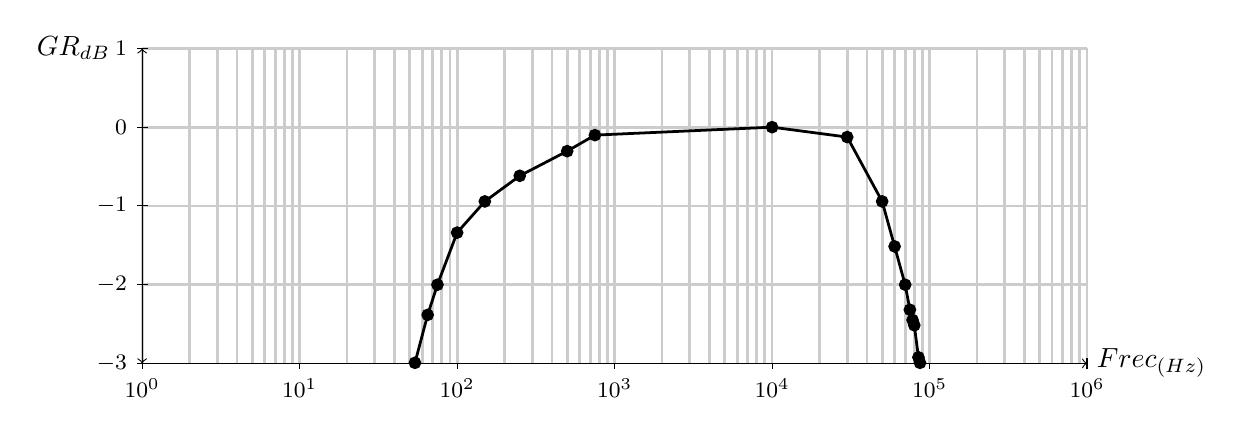
\begin{tikzpicture}[scale=1]

    \def\scalya{3}
    \def\scaly{1}
    \def\scalxa{3}
    \def\scalx{2}
    
    %datosLineaA
    \coordinate (a8) at ({log10(750)*\scalx},{20*log10(6.92/7)*\scaly+\scalya});
    \coordinate (a7) at ({log10(500)*\scalx},{20*log10(6.76/7)*\scaly+\scalya});
    \coordinate (a6) at ({log10(250)*\scalx},{20*log10(6.52/7)*\scaly+\scalya});
    \coordinate (a5) at ({log10(150)*\scalx},{20*log10(6.28/7)*\scaly+\scalya});
    \coordinate (a4) at ({log10(100)*\scalx},{20*log10(6.00/7)*\scaly+\scalya});
    \coordinate (a3) at ({log10(75)*\scalx},{20*log10(5.56/7)*\scaly+\scalya});
    \coordinate (a2) at ({log10(65)*\scalx},{20*log10(5.32/7)*\scaly+\scalya});
    \coordinate (a1) at ({log10(54)*\scalx},{20*log10(4.96/7)*\scaly+\scalya});
    \coordinate (a9) at ({(log10(10)+\scalxa)*\scalx},{20*log10(7.00/7)*\scaly+\scalya});
    \coordinate (a10) at ({(log10(30)+\scalxa)*\scalx},{20*log10(6.90/7)*\scaly+\scalya});
    \coordinate (a11) at ({(log10(50)+\scalxa)*\scalx},{20*log10(6.28/7)*\scaly+\scalya});
    \coordinate (a12) at ({(log10(60)+\scalxa)*\scalx},{20*log10(5.88/7)*\scaly+\scalya});
    \coordinate (a13) at ({(log10(70)+\scalxa)*\scalx},{20*log10(5.56/7)*\scaly+\scalya});
    \coordinate (a14) at ({(log10(75)+\scalxa)*\scalx},{20*log10(5.36/7)*\scaly+\scalya});
    \coordinate (a15) at ({(log10(78)+\scalxa)*\scalx},{20*log10(5.28/7)*\scaly+\scalya});
    \coordinate (a16) at ({(log10(80)+\scalxa)*\scalx},{20*log10(5.24/7)*\scaly+\scalya});
    \coordinate (a17) at ({(log10(85)+\scalxa)*\scalx},{20*log10(5.00/7)*\scaly+\scalya});
    \coordinate (a18) at ({(log10(87)+\scalxa)*\scalx},{20*log10(4.96/7)*\scaly+\scalya});



    
    %Ejex
    \foreach \x [evaluate={\a=int(\x+1)}]in {0,...,5}{
    \foreach \y in {1,...,10}
        \draw[line width=1pt,gray!40] ({(\x+log10(\y))*\scalx},0)--({(\x+log10(\y))*\scalx},4);
        \draw[shift={(\a*\scalx,0)}] (0pt,2pt) -- (0pt,-2pt) node[below] {\footnotesize $10^\a$};
    }
    \draw[shift={(0,0)}] (0pt,2pt) -- (0pt,-2pt) node[below] {\footnotesize $10^0$};
    \draw[->] (0,0)--(12,0) node[right] {$Frec_{(Hz)}$};
    
    %Ejey
    \foreach \y [evaluate={\a=int(\y-3)}] in {1,...,4}{
        \draw[line width=1pt,gray!40] (0,\y)--(12,\y);
        \draw[shift={(0,\y)}] (2pt,0pt) -- (-2pt,0pt) node [left] {\footnotesize $\a$};
    }
   \draw[shift={(0,0)}] (2pt,0pt) -- (-2pt,0pt) node [left] {\footnotesize $-3$};
   \draw[<->] (0,0)--(0,4) node[left=8pt]{$GR_{dB}$};
   
   
    %Linea A
    \foreach \x  in {1,...,18}{
        \draw[line width=1.5pt,fill=black] (a\x) circle(1.5pt);
   }
   \foreach \x [evaluate={\y=int(\x+1);}] in {1,...,17}{
        \draw[line width=1pt,black] (a\x) -- (a\y);
   }
   
\end{tikzpicture}